\documentclass{tufte-handout}
\title{Proposal – Product Team Metrics Wallboards}
\author{Laurent Lathieyre}

% Settings
  \date{December 2, 2023} % without \date command, current date is supplied
  %\geometry{showframe} % display margins for debugging page layout
  % Load the packages
  \usepackage{graphicx} % allow embedded images
    \setkeys{Gin}{width=\linewidth,totalheight=\textheight,keepaspectratio}
    \graphicspath{{graphics/}} % set of paths to search for images
  \usepackage{amsmath}  % extended mathematics
  \usepackage{blindtext}
  \usepackage{units}    % non-stacked fractions and better unit spacing
  \usepackage{multicol} % multiple column layout facilities
  \usepackage{lipsum}   % filler text
  \usepackage{booktabs} % For professional looking tables
  \usepackage{fancyvrb} % extended verbatim environments
    \fvset{fontsize=\normalsize}  % default font size for fancy-verbatim environments
  \usepackage{glossaries}
    \setacronymstyle{long-short}
  \usepackage{draftwatermark}
    \SetWatermarkScale{1}   
    \SetWatermarkLightness{0.95}
  
  % Standardize command font styles and environments
  \newcommand{\doccmd}[1]{\texttt{\textbackslash#1}}% command name -- adds backslash automatically
  \newcommand{\docopt}[1]{\ensuremath{\langle}\textrm{\textit{#1}}\ensuremath{\rangle}}% optional command argument
  \newcommand{\docarg}[1]{\textrm{\textit{#1}}}% (required) command argument
  \newcommand{\docenv}[1]{\textsf{#1}}% environment name
  \newcommand{\docpkg}[1]{\texttt{#1}}% package name
  \newcommand{\doccls}[1]{\texttt{#1}}% document class name
  \newcommand{\docclsopt}[1]{\texttt{#1}}% document class option name
  \newenvironment{docspec}{\begin{quote}\noindent}{\end{quote}}% command specification environment

%\makeglossaries % Generate the glossary
\loadglsentries{defns}

\begin{document}
\maketitle % this prints the handout title, author, and date
Last Update: December 8, 2023

\begin{figure}
    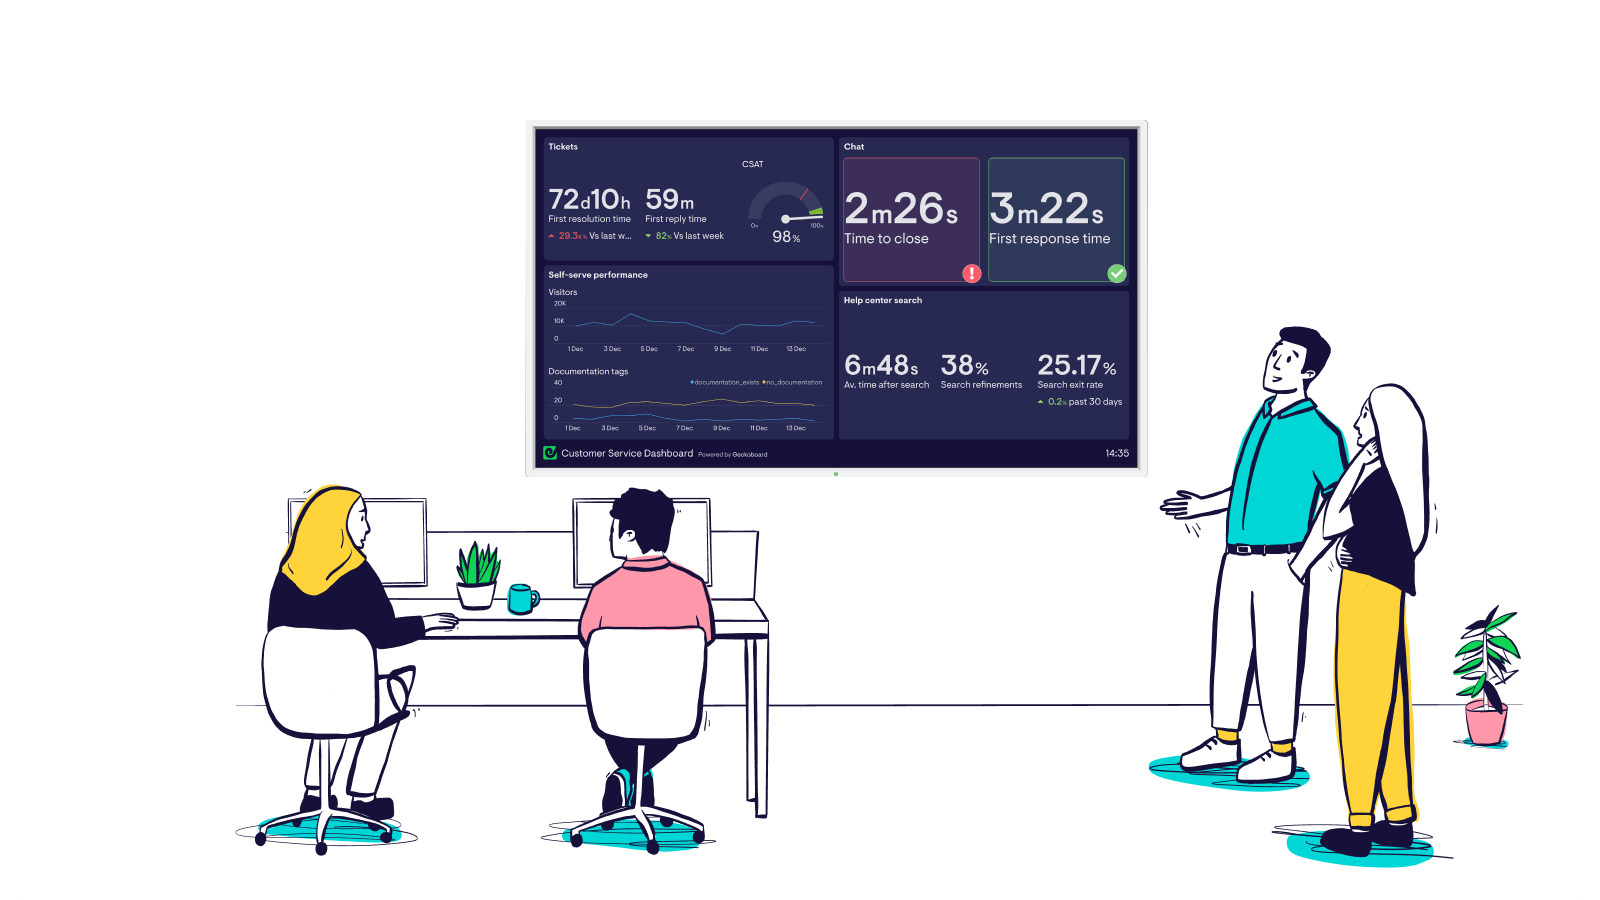
\includegraphics{share-tv.png}
\end{figure}

\section{Overview}\label{sec:overview}
  
\begin{marginfigure}[-80pt]
  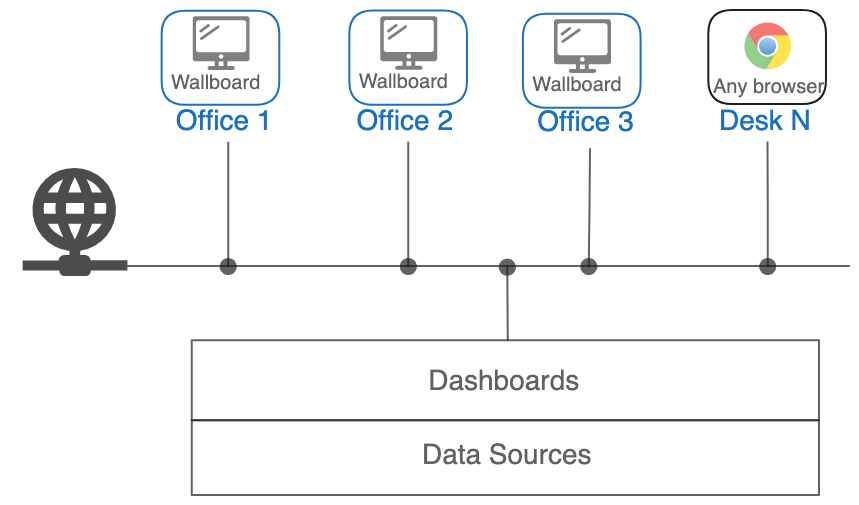
\includegraphics{Drawing 2023-12-01 15.06.45.excalidraw}
  \caption{Architecture Overview}
\end{marginfigure}

  \newthought{Shared metrics help Teams Focus and Teams Alignment.} This document is a proposal to implement \emph{Wallboards} for Sirion – a multi-office, multi-country, hybrid work environment.

  \par It is also part of the overaching effort to promote data litteracy\sidenote{Including awareness about statistical fallacies – the common tricks data can play on us, which lead to mistakes in data interpretation and analysis.}\cite{geckoboard-data-fallacies} and data driven decisions in the company.

\section{Overall Design}\label{sec:overall-design}
\newthought{One key fixture of this proposal is to use wall-mounted TV displays} with  a HDMI 2.0 port to connect a Raspberry Pi PC or other recommended small PCs such as a  MeLE PC Stick\cite{Amazoncom_B08LYRQZ59} or a Raspberry PI\cite{Raspberry-5} in high-traffic places (e.g. kitchen, water cooler, etc.) 
\par The dashboard automatically runs on all connected displays. 
\par Dasboard Loops are a great way to display several dashboards on a single screen. For example, we might want to display some company-wide metrics alongside our team’s existing dashboard, have a project-specific dashboard we need to keep an eye on, in addition to our day-to-day metrics, or have several teams who share a single screen. They are also accessible via a web browser\sidenote{Behind the company's \gls{sso}.}.

\section{Project Phasing}\label{sec:phasing}
\newthought{We want to use an iterative approach for this project to succeed – or to to fail fast!} The first phase – or \gls{poc} – will need approximately 2-month time from end to end.

\subsection{Phase 1}
  \begin{enumerate}
    \item Source Hardware and Software for 1 Display and Workstations access.
    \item Build one dashboard with 3 \gls{kpi}.
    \item Test it.
    \item Communicate with team members and run the experiment for 10-day.
    \item Get feedback.
    \item After Action Report.
  \end{enumerate}

\subsection{Phase 2}
\begin{enumerate}
  \item Extend to new metrics, and possibly to additional cross-functional Dashboards.
  \item Add new Displays and Workstation access.
  \item Kick-Off the official Launch.
  \item Measure. Evaluate. Adjust. Repeat.
\end{enumerate}

\section{KPIs}\label{KPIs}
We recommend to start with 3 simple \gls{smart} \gls{kpi}s such as
\begin{itemize}
%  \item Engagement \& Stickyness: Evolution of \gls{mau}, \gls{dau} and \gls{dau} \frac{\gls{mau}} ratio.
\item Engagement \& Stickyness: Evolution of \gls{mau}, \gls{dau} and $\frac{\gls{dau}}{\gls{mau}}$ ratio.
  \item User Satisfaction: Evolution of the \gls{nps}\sidenote{The set-up of a \gls{nps} campaign generation tool will have to be specifically addressed.}
  \item Feature Focus: for example
    \begin{itemize}
      \item A feature's activation funnel
      \item An A/B testing experiment
    \end{itemize}
\end{itemize}

\section{Key Success Factors}\label{key-success-factors}
\begin{itemize}
  \item Get \gls{slt} buy-in.
  \item Set a \gls{raci} matrix.
  \item Once the \gls{poc} is successful, institutionalize the project within the company (possibly hosted by a new team, have a \gls{sop} and documentation written-up.)
  \item Revisit the program and re-evaluate its \gls{roi} once a year.
\end{itemize}

\section{Budget Estimation}\label{sec:budget}
\begin{itemize}
  \item Phase 1 (approx. \$1,000)\sidenote{Does not include time spent; Assumes 3-month \gls{poc}.}
  \begin{itemize}
    \item Software Subscription \$300
    \item Display \$400
    \item Small PC  \$150
  \end{itemize}

  \item Phase 2 (approx. \$8,000) \sidenote{For 2 additional displays and 12-month run.}
  \begin{itemize}
    \item Software Subscription \$6,700
    \item +2 Displays w/PCs \$1,200
  \end{itemize}

\end{itemize}
\section{What Next?}\label{sec:what-next}
Once the above is successfully executed, and there is a wide adoption within the company, the suggested next phase is to implement a more rigorous approach in the use of data and the analysis of the evolution of \gls{kpi}s.
\par Amazon led the way on how to effectively use metrics in their business. The last chapter of "Working Backwards"\cite{Bryar2021} describes precisely the methodology used at Amazon. Some highlights can be found on the CommonCog website\cite{CommonCog2021}.
\subsection{Caveat}\label{sec:caveat}
Given that we are in a business-to-business type of software industry, the number of datapoints can range in the hundreds or thousands vs. millions for business-to-consumer activities. Hence one must remain attentive about the statistical significance of our data.
\subsection{Other Resources}\label{sec:resources}
\begin{itemize}
 \item Metrics that Matter to Product Managers (website)\cite{Holmes2017}
 \item Lean analytics: use data to build a better startup faster (book)\cite[+30pt]{croll_lean_2013}
 \item Although considered outdated or overkill by some people, I believe SixSigma – or its lighter version Lean SixSigma – is a very good methodology, training \& certification to understand key statistical concepts and put them in practice.
\end{itemize}

\pagebreak
\section{Guide to Product Metrics}
  \begin{table}[h]
    \centering
    \begin{tabular}{ll}
    \toprule
    \textbf{CATEGORY} & \textbf{METRIC} \\
    \midrule
    Acquisition & Number of new signups and/or qualified leads \\
                & Customer acquisition cost (CAC) \\
    Activation   & Activation rate \\
                & Time to activate \\
                & Free-to-paid conversions \\
    Engagement  & Monthly, weekly, and/or daily active users (MAU, WAU, DAU) \\
                & Stickiness (DAU/MAU) \\
                & Feature usage \\
    Retention    & Retention rate \\
                & Churn rate \\
                & Customer lifetime value (CLV) \\
    Monetization & Net revenue retention (NRR) \\
                & Monthly recurring revenue (MRR) \\
                & Average revenue per user (ARPU) \\
    North Star   & North Star Metric \\
    \bottomrule
    \end{tabular}
  \end{table}

\section{Example of Chart used at Amazon}\label{sec:amazon-chart}
  \begin{figure}
    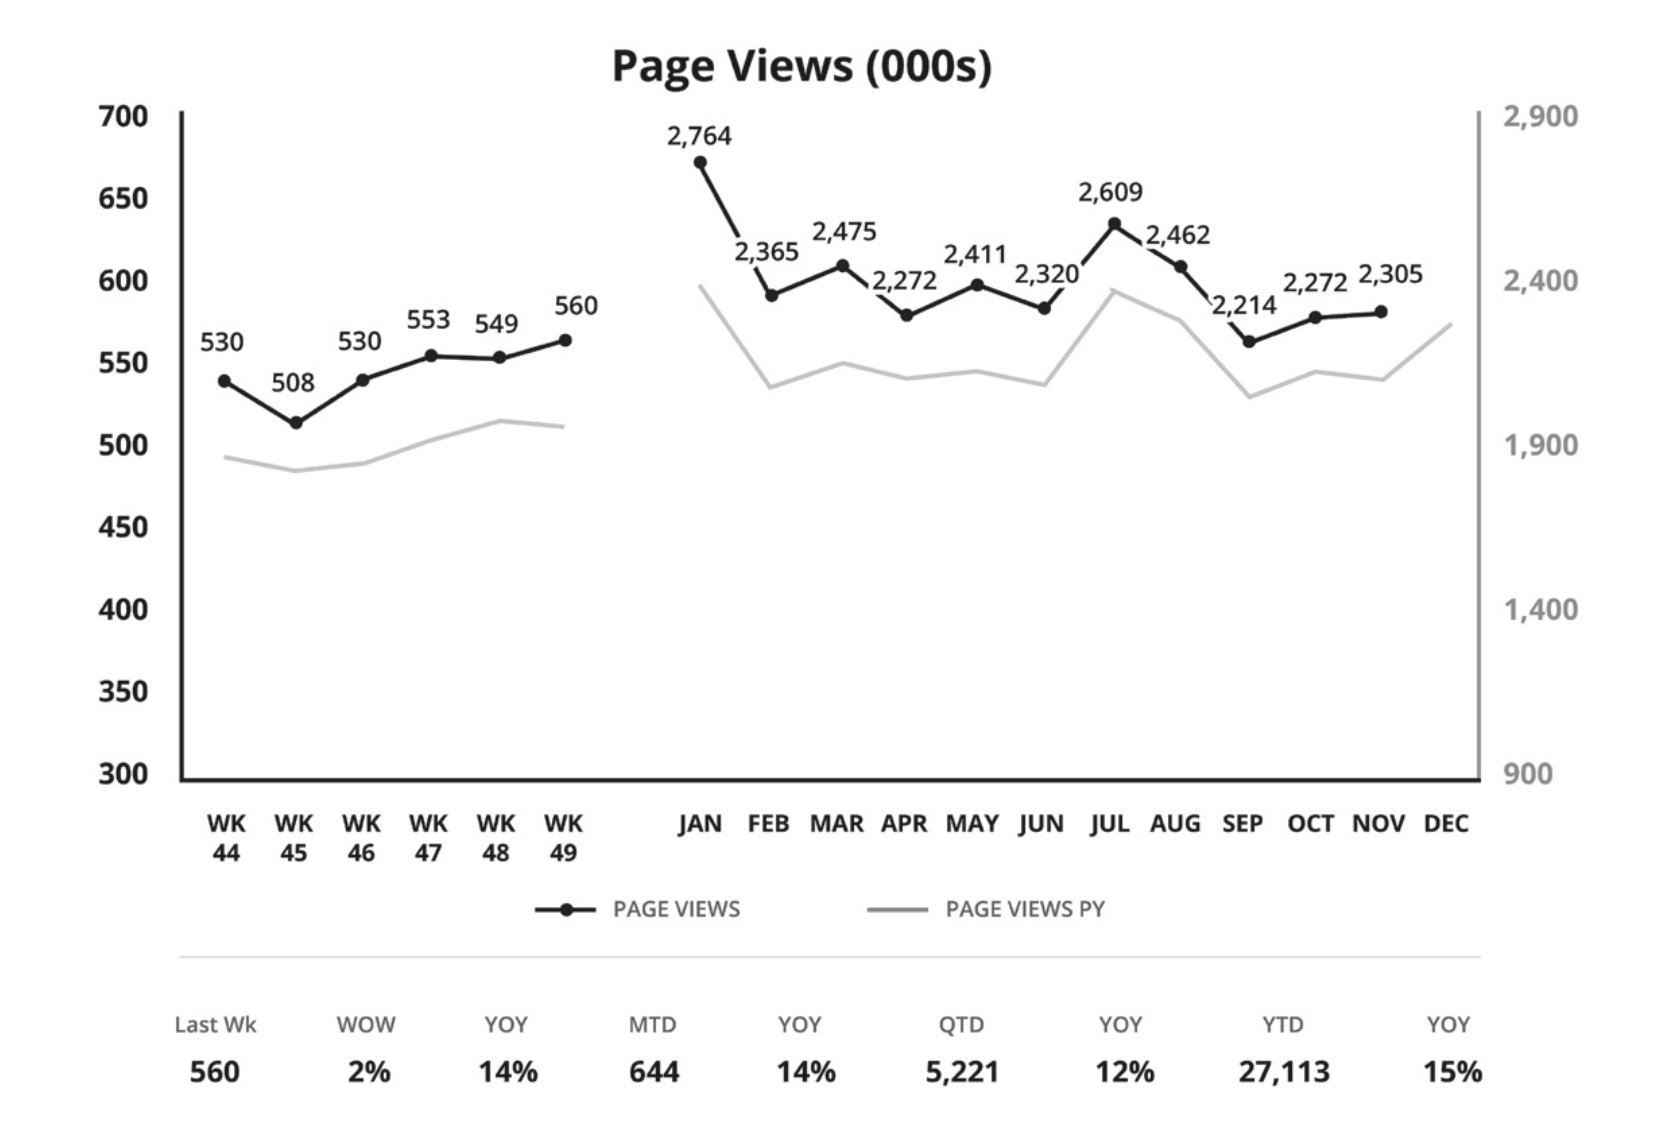
\includegraphics{amazon-page-views-chart.png}
  \end{figure}
  \par This graphic\cite{Bryar2021} measures page views for a business, and conveys a lot of data in a small space:
  \begin{itemize}
    \item{The gray line is prior year, the black line is current year}
    \item{The left graph, those first 6 data points, shows the trailing 6 weeks}
    \item{The right graph, with 12 data points, shows the entire trailing year month by month}
    \item{This built-in “zoom” adds clarity by magnifying the most recent data, which the 12-month graph puts into context.}
  \end{itemize}
  At the bottom of the chart, we call out additional key data points, most of which compare one period to another.

\newpage
\bibliography{MyReport-Product_Team_Dashboard}
\bibliographystyle{plainnat}

\end{document}